\section{Introduction}
The register-transfer level (RTL) programming model paved the road for Verilog and VHDL to flourish as the leading hardware description languages (HDLs) in the electronic design automation industry. However, that road is steadily nearing its end, as both hardware designs and devices become increasingly more complex. While the software world is striving for a "write once, run anywhere" programmability, an RTL design with the same requirements may vary greatly across different FPGA and ASIC devices that incorporate various technologies and core components. Moreover, minor requirement changes may lead to significant redesigns, since RTL abstraction prevents separation of functionality and timing constraints. For example, registers serve various roles such as preserving a state, pipelining and balancing a data path, deriving timed signals from an input clock, and synchronizing an input signal. This coupling between core requirements and device constraints leads to verbose and unportable RTL designs. 

Ongoing efforts to bridge this hardware programmability gap~\cite{Kapre2016, Nane2016, Windh2015} can be split into two major tracks: high-level synthesis (HLS) tools and high-level RTL (HL-RTL) languages.
On the one hand, HLS tools (such as Vivado~\cite{Vivado2012}, Catapult~\cite{graphics2008catapult}, and others~\cite{Kavvadias2013, synphony2015}) rely on modern programming languages like C or M and apply  auto-pipelining and optimization mechanisms to make hardware accelerators accessible to non-hardware engineers. While this approach has proven successful in algorithmic acceleration domains, such languages carry von Neumann sequential semantics and thus hinder construction of parallel hardware, which is required to describe architectures~\cite{Zhao2017}. Even a simple periodic led toggle is impossible to generate via HLS languages.
On the other hand, HL-RTL languages (such as Chisel~\cite{Bachrach2012}, Bluespec~\cite{nikhil2004bluespec}, PyRTL~\cite{Clow2017}, and others~\cite{Charles2016, Liu2017, jiang2018mamba, decaluwe2004myhdl, CxLang2014, Lockhart2014}) try to enhance productivity by introducing new hardware generation constructs and semantics but without abstracting over register-level description (even Bluespec that uses concurrent guarded atomic actions assumes rules complete within a single clock cycle). Therefore, HL-RTL designs are still subjected to the \emph{"tyranny of the clock"}~\cite{Sutherland2012} and are bound to specific timing and target constraints.

In this paper we propose a novel dataflow HDL abstraction layer that assimilates together constructs and semantics from dataflow\cite{le1986signal, Thuau1991}, hardware, and software programming languages to abstract over registers and clocks. We also introduce DFiant\footnote{A preliminary version of DFiant was first introduced as a poster. The reference was removed for blind review.}, a Scala-embedded HDL that utilizes this dataflow abstraction to decouple functionality from implementation constraints and thereby enable truely portable and composable hardware designs. The dataflow model offers implicit concurrency between independent paths while freeing the designer from explicit register placement that bind the design to fixed pipelined paths.  

\begin{figure*}[t]
	\centering
	\captionsetup{justification=centering}
	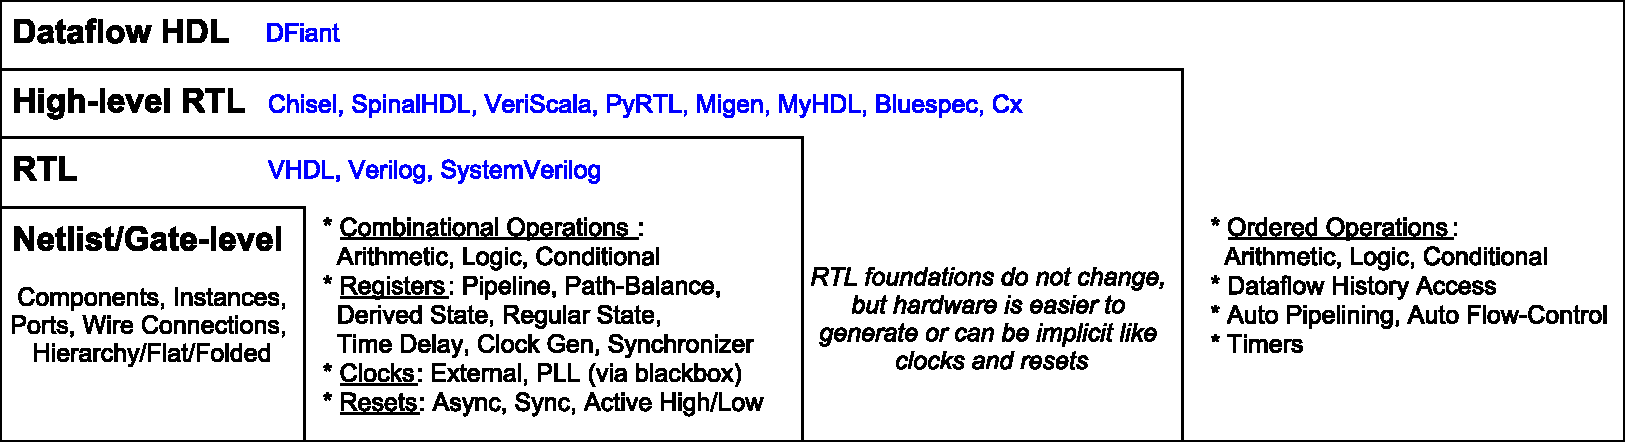
\includegraphics[width=\linewidth]{graphics/motivation.pdf} 
	\captionof{figure}{HDL abstraction layer summary (lowest=netlist, highest=dataflow) \\ DFiant is the first language to support the highest layer, a dataflow HDL.}
	\label{fig:motivation}
\end{figure*}

Recent related dataflow-for-hardware efforts are the Maxeler framework~\cite{Pell2011} and its MaxJ Java-based programming language, and the OpenDF framework~\cite{bhattacharyya2008opendf} which is based on the CAL actor language~\cite{eker2003cal}. MaxJ indeed carries common traits with DFiant, but it is tailored for its target hardware framework and does not fit as a general purpose HDL. The OpenDF framework shares similar goals with our work, but uses actors and networks to describe hardware, which is completely different than a conventional HDL composition based on component instances and port connections.

This work focuses on the DFiant language and compiler. DFiant is \emph{not} an HLS language, nor is it an RTL language, but it is still an HDL that provides abstractions beyond RTL behavioral modeling, to reduce verbosity yet maintain portable codes.
DFiant is implemented as a Scala library and therefore offers a rich type safe ecosystem along its own hardware-focused type system (e.g., bit-accurate dataflow types, input/output port types). The library performs two main tasks: first, the frontend compilation, which enforces the type-safe rule-system and constructs a dataflow dependency graph; and second, the backend compilation, which translates the graph into a pipelined RTL code and a TCL constraints file, followed by a hardware synthesis process using commercial tools. 

The paper is organized as follows. The next section clarifies the motivation behind the dataflow HDL abstraction layer, followed by Section~\ref{sec:dfiant}, which provides a general overview of the DFiant HDL language. 
Section~\ref{sec:evaluation} describes our evaluation of the DFiant language and compiler, and finally, Section~\ref{sec:conclusion} concludes the paper.


%Interactions between DFiant types lead to hardware construction, while non-DFiant types (e.g. Integer) are considered as constants. 
 